\documentclass[a4paper, 12pt]{article}

\usepackage[utf8]{inputenc}
\usepackage{graphicx}
\usepackage{nameref}
\usepackage[hyphens]{url}
\usepackage{hyperref}
% These two packages are for setting up code segments in the document
\usepackage{listings}
\usepackage{color}

% define some colours
\definecolor{dkgreen}{rgb}{0,0.6,0}
\definecolor{gray}{rgb}{0.5,0.5,0.5}
\definecolor{mauve}{rgb}{0.58,0,0.82}
\definecolor{backcolour}{rgb}{0.95,0.95,0.92}

% set the style of your code segments
\lstset{
    %frame=tb,
    language=bash,
    backgroundcolor=\color{backcolour},
    aboveskip=3mm,
    belowskip=3mm,
    showstringspaces=false,
    columns=flexible,
    basicstyle={\small\ttfamily},
    numbers=none,
    numberstyle=\tiny\color{gray},
    keywordstyle=\color{blue},
    commentstyle=\color{dkgreen},
    stringstyle=\color{mauve},
    %breaklines=true,
    %breakatwhitespace=true,
    %tabsize=3
}

\begin{document}

\part*{Version Control using Git/GitHub}

\section*{Basic Intro to Version Control System}

The point of having a version control system is to make things easier for you to keep track of all the changes you  have made to your document.
This image shows a nightmare situation you may end up in while writing a thesis:\\
\begin{center}

\includegraphics[width=0.8\textwidth]{./images/index}
\end{center}

The point of this image is to show that it is hard for you to keep track of all the changes you or someone else has made to a document, especially when all the changed files are so similar to one another.
Yes, Microsoft Word and Google Docs may have those "track changes" and comments functionality that makes them somewhat easier to work with, but if you're working with codes or plain text files (for example R scripts and \LaTeX{} documents), MS word is useless.

Also, what if you want to track multiple files that are important for the project?
How would you keep track of all the changes and keep everything up to date?
How are you going to go back to your old copy/version of your project or document?
Are you going to back up all the files every time someone changes a line?
If you think you can do all of this manually, go for it!
I'm not saying it's impossible, but it will be hard work (and things will get messy real quick).

An alternative to this is to use a version control system (VCS) such as Git.
With a VCS, you will start off with a base document (i.e. ``original'' copy of the document) to keep track of.
Each time you make a change to your document, VCS keeps track of the changes made to the document.
%check if fork/merge is correctly used
If you have one or more people editing a document, you can copy (or ``fork'') the base document and make changes to it, and once you're happy with it, you can then combine your changes and the changes the other person have made to the document into a single document (which is called ``merging'').\\
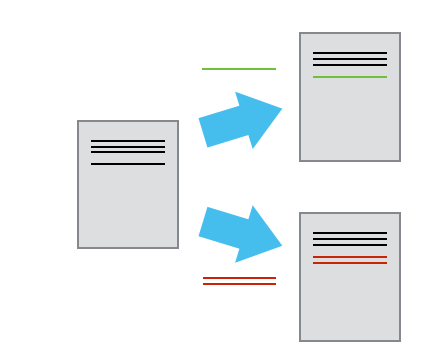
\includegraphics[width=0.5\textwidth]{./images/versions}
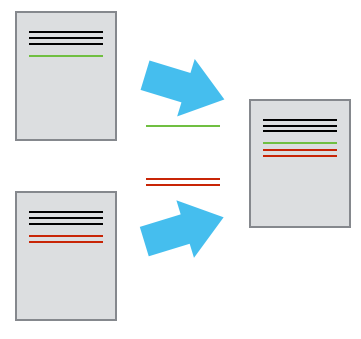
\includegraphics[width=0.42\textwidth]{./images/merge}

Another advantage of using  a VCS is that you can always ``roll back'' to the specific document file at any time.
In other words, you can go back to your older version of the document (hence ``version control'' system).

We will be using Git and GitHub as an example program to show how VCS is used, both locally and remotely.

\section*{Setting up Git on your computer}

Before we can use Git on the computer, you need to configure it a little:

\begin{lstlisting}
$ git config --global user.name "your_username"
$ git config --global user.email "your_email"
\end{lstlisting}
You can check the settings anytime by typing:

\begin{lstlisting}
$ git config --list
\end{lstlisting}

\section*{Creating a Repo}

A repository (or ``repo'') is a file/directory where you want Git to track changes of all your documents.
To create a repo, go to the directory you want to track changes and type:

\begin{lstlisting}
$ git init
\end{lstlisting}
This will create an invisible file \verb|.git| in your directory:

\begin{lstlisting}
$ ls -a
.   ..  .git
\end{lstlisting}
In general, it is not a good idea to make a repo within a repo.
Also, you don't want to keep track of the files that are not related to your project.
As a general rule of thumb, you should create a repository as high up in the directory as you can for that project, without having to track unnecessary files.

\section*{Tracking changes}

Once a repo is created/initiated, you can add/edit/remove files into your repo.
You can check what kind of changes you have made to the repo:
\begin{lstlisting}
$ git status
\end{lstlisting}
This shows which files have been added/modified/removed from the repo.
To make Git to track the changes you have made to your repo, you have to tell git that you have added some changes to the repo:
\begin{lstlisting}
$ git add .
\end{lstlisting}
After adding the changes, Git will notice that this repo is slightly different from the original repo, and there are changes to be ``committed''.
This means that git hasn't recorded your changes to the project just yet and require you to commit and save the changes you have made to the repo.
To do this, type:
\begin{lstlisting}
$ git commit -m 'I have edited my repo'
\end{lstlisting}
The \verb|-m| flag is short for message, and the message that we type in between the quote marks make it easier for us to look for certain changes when we want to go back to it.
After \verb|git commit| command, all the changes are saved:
\begin{lstlisting}
$ git status
# On branch master
# nothing to commit, working directory clean
\end{lstlisting}
This shows us that everything is up to date.
To see what we have changed in the past (i.e. the commits we have made in the past), we can use:
\begin{lstlisting}
$ git log
# commit: <some_random_identifier>
# Author: your_username <your_email>
# Date: date_and_time_of_your_commit
# 
# <Message you wrote when you committed the changes>
\end{lstlisting}
If you want to look at the changes before you add/commit the changes you have made, you can use:
\begin{lstlisting}
$ git diff
\end{lstlisting}

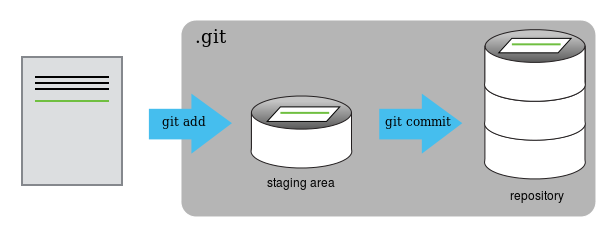
\includegraphics[width=0.9\textwidth]{./images/staging}
\\Looking a little bit more into the details, in the process of committing changes with Git, there is a thing called the staging area.
This staging area is where all the changes to be committed are tracked, but not yet ready for commit.
Once everything is ready (for example your program is running, or you've made enough edits to your document for proof reading), you can commit and save all the changes you have made and permanently store it in the repo.

So, what you're doing with \verb|git add| is putting all the changes to the staging (draft/working) area, and then \verb|git commit| saves all the changes into the repo (good copy/version).

\section*{Looking back at the commit history}

As mentioned earlier, \verb|git log| will let you see what commits we have made in the past.
\verb|git diff <commitID or relative_to_HEAD> [file]| allows us to look at the difference between the particular commit version of the \verb|file| with the current version.

If we wanted to roll back to an older version, we can use:
\begin{lstlisting}
$ git checkout branch_name OR <commitID or relative_to_HEAD> [file]
\end{lstlisting}
to have a look (``chekout'' the particular commit/file/branch).
This creates a ``detached'' repo to work with, and you can do whatever you want.
If you then decided to keep the changes you have experimented with, you'll have to make a ``branch'' first, then ``merge''it.
To make a new branch, you  type:
\begin{lstlisting}
$ git branch <name_of_branch>
\end{lstlisting}
To see what branches you currently have, type:
\begin{lstlisting}
$ git branch
\end{lstlisting}
To switch branches, use the checkout command:
\begin{lstlisting}
$ git checkout name_of_branch
\end{lstlisting}
If you know that you are going to make changes to the previous commit and merge it with the original branch, then you can make a branch from the previous commit:
\begin{lstlisting}
$ git checkout <commitID or relative_to_HEAD> -b <name_of_branch>
\end{lstlisting}
The \verb|-b| flag tells the command to make a new branch with the specified branch name.
Once you're done with all the changing and ready to merge with the master branch, type:
\begin{lstlisting}
$ git merge <branch_to_be_merged>
\end{lstlisting}
This command will merge the changes in the current branch with the ``branch\_to\_be\_merged''.
For example, if you do the following command in the master branch:
\begin{lstlisting}
$ git merge test
\end{lstlisting}
It will merge/add the changes from test into the master branch.

\section*{Ignoring specific filetypes}

It is a good idea to track changes of only the essential files, and no other files (for example, track changes of the codes, but not your original data).
You can specify which filetypes to be tracked or not by configuring the \verb|.gitignore| file (which you will have to make yourself).
Any filetypes included in the \verb|.gitignore| file (including directories) will be ignored by Git for tracking changes.

\section*{Remote repo with GitHub}

So we have looked at how to create a repo, how to commit, roll back and merge branches.
Next step is to centralise the files on the web so you can access your files from anywhere.
To do this, we'll use GitHub, which will essentially act as like a dropbox folder, but with version control system built in to it.

First, you need to create a new repo on GitHub  website.
This repo will have no files or directories, so we will have to ``push'' our {\itshape local} repo onto this {\itshape remote} repo.

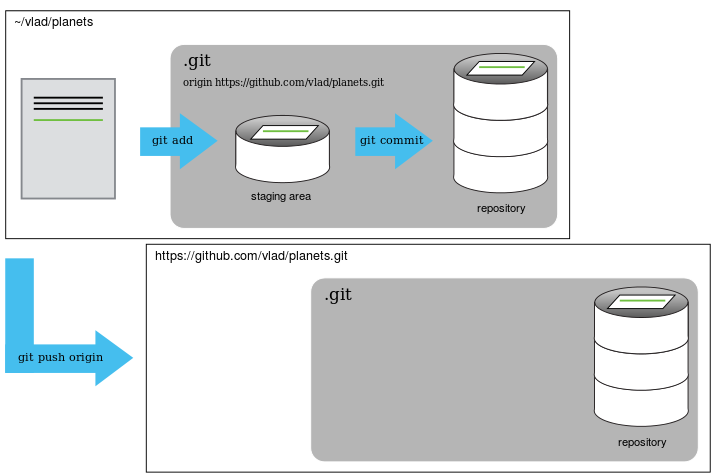
\includegraphics[width=0.9\textwidth]{./images/github}
\\To push your local repo onto the remote repo, type:
\begin{lstlisting}
$ git remote add origin <URL_to_your_remote_repo>
$ git push origin master
\end{lstlisting}

Now the local and the remote repo is connected - you can change the files on your local repo and push it onto the remote repo, or you can pull the changes from the remote repo onto your local repo.
NOTE: always pull first, before you push to a remote repo.
This will update your local repo to the newest version first, then push the changes to the remote repo.

\section*{Download an already existing repo}
\label{sec:clonerepo}

To download an already existing repo (whether it's yours or someone else's), type:
\begin{lstlisting}
$ git clone <URL_to_remote_repo>
\end{lstlisting}
This will download the repo specified by the URL.
You can now push and pull from this remote repo (unless if it's another person's repo, in which case you can only pull from them - you'll need a special permission from them to push to the repo).

\section*{Using SSH instead of HTTPS}

When you use HTTPS to access the remote GitHub repo, you'll have to type in your username and passsword each time you want to push to that repo, which could be annoying at times.
An alternative to this is to clone your repo using the SSH URL instead of the HTTPS URL.
SSH protocol allows you to push and pull your local repo to your remote repo without having to type in your username or password.
To use the SSH with Git/GitHub, you have to generate a SSH key on your computer and send the public key to GitHub.

\subsection*{Public and Private key pair}

When you make a SSH key, you generate a {\itshape public} key and a {\itshape private} key.
SSH is a protocol in which you access the remote computer from your host computer in a secure manner.
To do this securely, the host computer holds onto a private SSH key, which is paired up with the public SSH key on the remote computer, and to access the remote computer, you need your private key that is paired up with the public key on the remote computer.
Without the matching key pair, you cannot access the remote computer.

What we are about to do with GitHub is something similar: we're going to generate the SSH key pair, then provide GitHub with our {\bfseries public} key only, so that we can access our repo in a secure manner.

\subsection*{Checking for existing SSH keys}

Open your terminal and type:
\begin{lstlisting}
$ ls -al ~/.ssh
\end{lstlisting}
By default, the filenames of the public keys are one of the following:
\begin{itemize}
\item[-] id\_dsa.pub
\item[-] id\_ecdsa.pub
\item[-] id\_ed25519.pub
\item[-] id\_rsa.pub
\end{itemize}

If you already have a public key, skip to {\itshape \nameref{sec:addssh}}.
If you don't have a public key, just keep reading.

\subsection*{Generate a new SSH key}

Open a terminal and type:
\begin{lstlisting}
$ ssh-keygen -t rsa -b 4096 -C "your_email"
# Generating public/private rsa key pair.
# Enter a file in which to save the key (/home/riku/.ssh/id\_rsa): 
[Press enter]
# Enter passphrase (empty for no passphrase): [Type a passphrase]
# Enter same passphrase again: [Type passphrase again]
\end{lstlisting}
The \verb|-t| flag specifies what type of SSH key we are generating (in this case rsa), \verb|-b| flag specifies how many bits are used in the key (4096 bits), and the \verb|-C| flag is for commenting your email.
The file in which the key is getting saved should be in the .ssh/id\_rsa file in your home directory.
Type in a passphrase (note: passphrase can contain whitespaces, unlike passwords).

\subsection*{Add SSH key to GitHub}
\label{sec:addssh}

Before adding a new (or existing) SSH key to GitHub, you need to add it to your ssh-agent:
\begin{lstlisting}
$ eval "$(ssh-agent -s)"
# Agent pid *****
$ ssh-add ~/.ssh/id_rsa
\end{lstlisting}
The first \verb|eval| command makes sure that the ssh-agent is running, and the \verb|ssh-add| command adds the private key to the agent (replace the id\_rsa with a different key, if you already have a SSH key).

To add the public SSH key to GitHub, you need to copy ALL of the text in the id\_rsa.pub file to your clipboard (i.e. ctrl-c).
Go to GitHub and log in.
Go to Settings \textgreater SSH keys \textgreater New SSH key, fill in the title field, and paste your public key into the key field, then click Add SSH key.
Confirm it by entering your GitHub password.

To confirm that you've added your SSH key to your account, type:
\begin{lstlisting}
$ ssh -T git@github.com
\end{lstlisting}
Type in ``yes'' if you're asked if you want to continue connecting, and then type in your passphrase for the SSH key (not your GitHub password).\\
If you get a message like this, you're all set for SSH access to remote repo:
\begin{lstlisting}
# Hi username! You've successfully authenticated, but GitHub does
# not provide shell access.
\end{lstlisting}

\section*{Forking a repo and issue pull requests}

So, the problem with contributing to an already existing repo is that you can't make changes to the repo, unless you are specifically named as one of the contributers of that project.
One way to contribute to the repo is by {\itshape forking} the repo into your account, then make changes to it through your account, then issuing a {\itshape pull request} so the project leader can merge the changes you have made (if it's good enough).

\subsection*{Fork a repo on GitHub}

First step is to fork the original repo you want to contribute to on GitHub.
Go to GitHub and navigate yourself to the repo you are interested in, and click the ``Fork'' button on the top right hand corner.
You should now have a copy of the original repo in your account.

\subsection*{Clone your fork onto your local machine}

This should be quite straightforward, as we have already gone through how to do this in the {\itshape \nameref{sec:clonerepo}} section.
Copy the SSH/HTTPS URL on GitHub and clone it using the \verb|git clone| command:
\begin{lstlisting}
$ git clone <your_fork_url>
\end{lstlisting}

Now you have a copy of the repo remotely on your GitHub account, and another copy of the repo on your local machine.
Since the repo is a forked version of the original repo on {\itshape your} account, you can make any changes you want and add/commit/push/pull as much as you like.

\subsection*{Keeping your repo up to date with the original repo}

While you are making changes to the forked repo, the project will carry on and there may be new changes in the original repo  which you may not be aware of.
To keep your forked repo up to date with the original repo, you need to add the original repo to the list of remote repos you are pulling/getting contents from.

\begin{center}
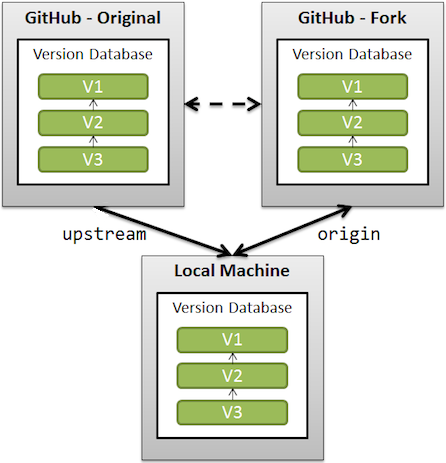
\includegraphics[width=0.7\textwidth]{./images/fork}
\end{center}

{\scriptsize See: \url{http://stackoverflow.com/questions/9257533/what-is-the-difference-between-origin-and-upstream-in-github/9257901#9257901 } \\}

The idea here is to have your forked repo to make your personal changes, and an ``upstream'' original repo to keep yourself up to date with the project.
Once your forked repo is good enough, then you can send a pull request and get the two merged (see {\itshape \nameref{subsec:sendpullrequest}}).

In terminal, go to your local repo directory and check what remote repo you have for the current fork:
\begin{lstlisting}
$ git remote -v
# origin <fork_URL> (fetch)
# origin <fork_URL> (push)
\end{lstlisting}
To make an upstream repo, you will have to copy the URL from the original repo as in {\itshape \nameref{sec:clonerepo}}.
Now, type:
\begin{lstlisting}
$ git remote add upstream <orignal_repo_URL>
$ git remote -v
# origin    <fork_URL> (fetch)
# origin    <fork_URL> (push)
# upstream  <original_repo_URL> (fetch)
# upstream  <original_repo_URL> (push)
\end{lstlisting}
Now you have both the upstream repo and your forked repo to pull/fetch codes from.
To fetch/update your repo with the original repo:
\begin{lstlisting}
$ git fetch upstream
\end{lstlisting}
This will create a new branch called ``upstream/master'', which you will have to merge it with your ``master'' branch to fully update your forked repo.
You will have to change to your master branch:
\begin{lstlisting}
$ git checkout master
# Switched to branch 'master'
$ git merge upstream/master
\end{lstlisting}
After this, your master branch (i.e. your forked repo) will be up to date with the original repo and you can carry on editing/hack away at your forked repo (remember to push the changes after updating).

\subsection*{Sending pull requests to merge your changes with the original repo}
\label{subsec:sendpullrequest}

Now we can change everything and anything on our forked repo, but what if you want your changes to be made permanent in the original repo that you have forked from?
You can change your forked repo, but you still can't push your changes onto the original repo.
This is when you issue a pull request, so that the project manager can review the changes and pull the changes you have made.

To do this, go to your GitHub account and navigate to your forked repo, then click on ``New pull request''.
Review your pull request, then send the pull request by clicking on ``Create pull request''.

















\end{document}
